\documentclass[12pt,a4paper]{article}
\RequirePackage{etex}
\usepackage{inputenc}
\usepackage[spanish]{babel}
\usepackage{amsmath}
\usepackage{amsthm}
% \usepackage{mathtools}
\usepackage{amsfonts}
\usepackage{graphicx}
\usepackage{fourier-otf}
\usepackage{physics}
\usepackage{wrapfig}
\usepackage{multicol}
\usepackage{caption}
\usepackage{subcaption}
\usepackage{hyperref}
\usepackage[left=2cm,right=2cm,top=2cm,bottom=2cm]{geometry}
\usepackage{tikz}

\newtheorem{theorem}{Teorema}
\usetikzlibrary{shapes, automata, arrows}


\title{Inferencia en redes bayesianas}
\author{Francisco J. Palmero Moya}
\date{Enero 2022}

% \renewcommand{\labelenumi}{(\alph{enumi})}
\begin{document}
\renewcommand{\tablename}{Tabla}

\maketitle

\paragraph*{Ejercicio 2.1}
Sea la red bayesiana

\begin{figure}[h!]
    \centering
    \begin{tikzpicture}[main/.style = {draw, circle}] 
        \node[main] at (0, 5) (A) {A};
        \node[main] at (-1, 3) (B) {B};
        \node[main] at (1, 3) (C) {C};
        \node[main] at (0, 1) (D) {D};
        \node[main] at (2, 1) (F) {F};
        \node[main] at (-2, 1) (G) {G};

        \draw [-to] (A) -- (B);
        \draw [-to] (A) -- (C);
        \draw [-to] (B) -- (D);
        \draw [-to] (C) -- (F);
        \draw [-to] (D) -- (F);
        \draw [-to] (D) -- (G);
        \end{tikzpicture} 
    \caption{Red bayesiana}\label{fig:red}
\end{figure}
y las probabilidades asociadas del enunciado. Se cumple que 
\begin{align}
    P(+b , +f, \neg g) & = \sum_{a, c, d} P(a, +b, c, d, +f, \neg g) \\
    P(+f, \neg g) & = \sum_{b} \sum_{a, c, d} P(a, b, c, d, +f, \neg g) = \sum_{b} P(b , +f, \neg g) \\
    P(+b | +f, \neg g) & = \frac{P(+b , +f, \neg g)}{P(+f, \neg g)} \label{eq:f}
\end{align}
Se tiene que
\begin{align}\label{eq:fac}
    P(+b , +f, \neg g) & = \sum_{a, c, d} P(a, +b, c, d, +f, \neg g) \\
    & = \sum_{a} \sum_{c} \sum_{d} P(a) P(+b | a) P(c | a) P(d | +b) P(+f | c, d) P(\neg g | d)
\end{align}
Solo por aclarar la notación, las variables de la red son binarias y,por tanto, el sumatorio sería sobre $a, b, c \in \left\{+, \neg \right\}$. Utilizando el método de la fuerza bruta, esto daría lugar a $2^3 = 8$ sumandos, cada uno de ellos obtenido tras realizar 5 multiplicaciones.\\

Veamos como se puede realizar el cálculo anterior mediante el \textbf{método de eliminación de variables}. Tomamos la variable $D$ y reunimos todos los potenciales que dependen de ella
\begin{align*}
    \psi_1(c) & = \sum_d P(d | +b) P(+f | c, d) P(\neg g | d) \\
    & = P(+d | +b) P(+f | c, +d) P(\neg g | +d) + P(\neg d | +b) P(+f | c, \neg d) P(\neg g | \neg d) \\
    & = 0.6*0.6*P(+f | c, +d) + 0.4*0.9*P(+f | c, \neg d)
\end{align*} 
Sustituyendo los valores que puede tomar $C$
\begin{align*}
    \psi_1(+c) & = 0.6*0.8*0.6+0.4*0.6*0.9 = 0.504   \\
    \psi_1(\neg c) & = 0.6*0.5*0.6+0.4*0*0.9 = 0.18
\end{align*}
Se obtiene así 
\begin{align*}
    P(+b , +f, \neg g) = \sum_{a} \sum_{c} P(a) P(+b | a) P(c | a) \psi_1(c)
\end{align*}
Pasamos ahora a calcular el segundo potencial
\begin{align*}
    \psi_2(a) & = \sum_c P(c | a) \psi_1(c) \\
    & =  P(+c | a) \psi_1(+c) + P(\neg c | a) \psi_1(\neg c) \\
    & = 0.504*P(+c | a) + 0.18*P(\neg c | a)
\end{align*}
Sustituyendo los valores que puede tomar $A$
\begin{align*}
    \psi_2(+a) & = 0.504*0.75+0.18*0.25 = 0.423 \\
    \psi_2(\neg a) & = 0.504*0.25 + 0.18*0.75 = 0.261
\end{align*}
Hemos eliminado así la variable $C$, lo que da lugar a
\begin{align*}
    P(+b , +f, \neg g) = \sum_{a} P(a) P(+b | a) \psi_2(a)
\end{align*}
Finalmente, eliminamos la variable $A$
\begin{align*}
    P(+b , +f, \neg g) & = P(+a) P(+b | +a) \psi_2(+a) + P(\neg a) P(+b | \neg a) \psi_2(\neg a) \\
    & = 0.3*0.9*0.423+0.7*0.2*0.261 = 0.15075
\end{align*}
Hay que tener en cuenta que esta probabilidad, equivale a sustituir $b=+b$ en el potencial que estamos calculando $\psi_3(b) = P(b, +f, \neg g)$. Por otro lado,
\begin{align*}
    P(+f, \neg g) & = \sum_b P(b, +f, \neg g) = P(+b, +f, \neg g) + P(\neg b, +f, \neg g)\\
    & = \sum_b \psi_3(b) = 0.15075 + \left[ 0.3*0.1*0.423 + 0.7*0.8*0.261 \right] \\
    & = 0.15075 + 0.15885 = 0.3177
\end{align*}
La probabilidad buscada es, usando la ec. \eqref{eq:f}
\begin{align*}
    P(+b | +f, \neg g) & = \frac{P(+b , +f, \neg g)}{P(+f, \neg g)} = \frac{0.15075}{0.3177} \simeq 0.5
\end{align*}

\paragraph*{Ejercicio 2.2}
Sea la red bayesiana del ejercicio anterior y las mismas probabilidades asociadas, vamos a realizar los cálculos usando OpenMarkov.

Los pasos seguidos son los siguientes:
\begin{enumerate}
    \item Definir los nodos y sus enlaces. Véase Figura \ref{fig:bn}.
    \item Definir las tablas de probabilidad correspondientes a cada uno de los nodos.
    \item Introducir los hallazgos. Véase Figura \ref{fig:inf}.
\end{enumerate}
Aunque los resultados difieren ligeramente, suponemos que es por errores de redondeo o porque el método de inferencia de OpenMarkov no es exacto.
\newpage
\begin{figure}[h!]
    \centering
    \begin{subfigure}{\textwidth}
        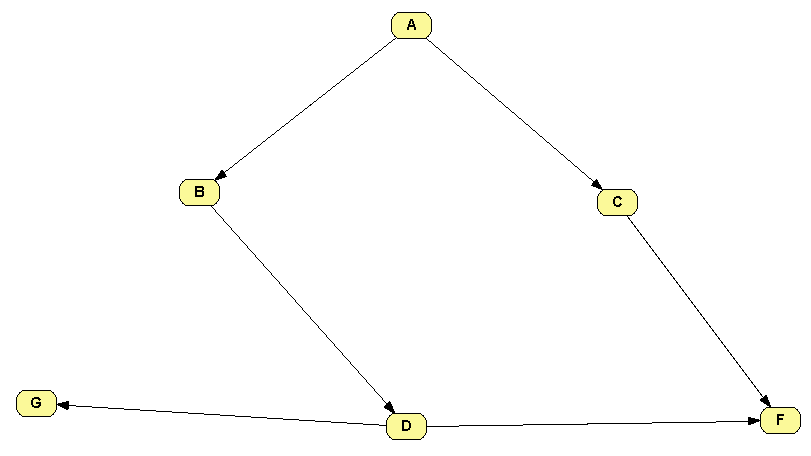
\includegraphics[width=\textwidth]{bn.png}
        \caption{Red bayesiana}
        \label{fig:bn}
    \end{subfigure}
    \hfill
    \begin{subfigure}{\textwidth}
        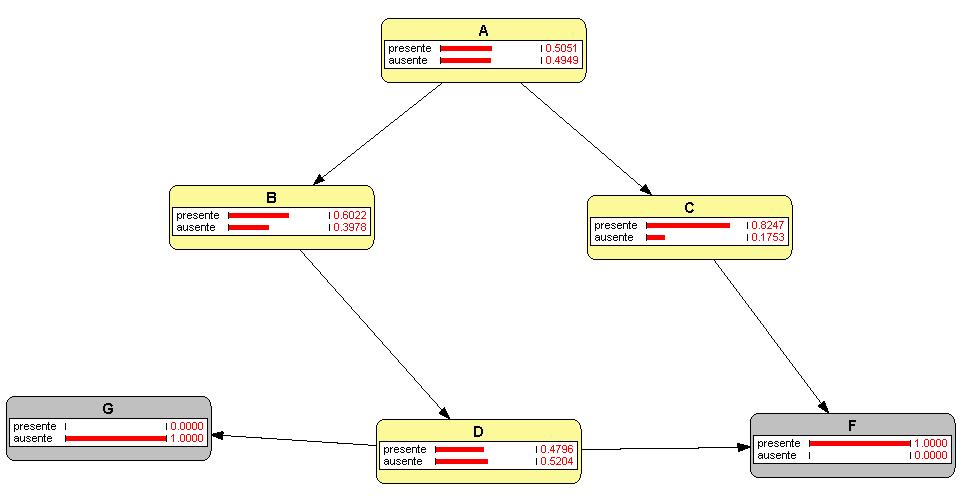
\includegraphics[width=\textwidth]{inf.png}
        \caption{Inferencia con hallazgos}
        \label{fig:inf}
    \end{subfigure}
    \caption{Solución Ejercicio 2.2}
\end{figure}

\paragraph*{Ejercicio 2.3}
Los métodos estudiados con anterioridad son métodos exactos, i.e., calculan las probabilidades condicionales de los nodos de forma exacta. Se ha demostrado (véase Cooper (1990)) que este tipo de tarea de propagación exacta es NP-compleja. \\
Surgen así los métodos de propagación aproximada donde la idea básica consiste en generar una muestra de tamaño $N$, a partir de la función de probabilidad conjunta de las variables, y luego utilizar la muestra generada para calcular valores aproximados de las probabilidades de ciertos sucesos dada la evidencia. Estas probabilidades se aproximan mediante los cocientes de la frecuencia de aparición de los sucesos en la muestra y el tamaño de la muestra.\\

Vamos a hacer un estudio de los pasos a seguir en los siguientes métodos aproximados para calcular la probabilidad anterior:

\begin{description}
    \item[Muestreo lógico] Se trata de un método de simulación en el que se pretende calcular la distribución de probabilidad real a partir de una distribución simulada. Este método se conoce como método aceptación-rechazo y se puede fundamentar en el siguiente teorema.
    \begin{theorem}[El método de aceptación-rechazo]
        Sea $X$ una variable aleatoria con función de probabilidad $p(x)$. Supóngase que $p(x)$ puede ser expresada como 
        \begin{align}
            p(x) = c g(x) h(x)
        \end{align}
        donde $c \geq 1, 0 \leq g(x) \leq 1$ y $h(x)$ es uan función de probabilidad. Sea $U$ una variable aleatoria uniforma $U(0, 1)$ y sea $Y$ una variable aleatoria con función de probabilidad $h(y)$ independiente de $U$. Entonces, la función de probabilidad condicional de $Y$ dado que $u \leq g(y)$ coincide con la función de probabilidad de $X$. Por otra parte, la probabilidad de aceptar la muestra es $1/c$.
    \end{theorem}

    El método de aceptación-rechazo para nuestro caso, genera las variables una a una de forma que se muestra una variable sólo cuando ya han sido muestreados todos sus padres. Según este método se simulan todas las variables, incluyendo las evidenciales.

    Sea la red bayesiana de la Figura \ref{fig:red}. La función de probabilidad conjunta puede factorizarse como en \eqref{eq:fac}. Los pasos a seguir son:
    \begin{enumerate}
        \item Muestreo de la variable $A$: Se consulta un generador de muestras aleatorios que, basándose en la distribución de probabilidad $P(a)$, de $+a$ con probabilidad 0.3 y $\neg a$ con probabilidad 0.7. Seguidamente se utiliza este valor $\hat{a}_1$ para calcular las probabilidades de los restantes nodos de extracción. 
        \item Muestreo de la variable $B$: dado $A=\hat{a}_1$, se consulta la probabilidad condicionada $P(b | \hat{a}_1)$ y se genera una muestra aleatoria con las correspondientes probabilidades. Supóngase que dicho valor para $B$ resulta ser $\hat{b}_1$. 
        \item Muestreo de la variable $C$: dado $A=\hat{a}_1$, se consulta la probabilidad condicionada $P(c | \hat{a}_1)$ y se genera una muestra aleatoria con las correspondientes probabilidades. Supóngase que dicho valor para $C$ resulta ser $\hat{c}_1$. 
        \item Muestreo de la variable $D$: dado $B=\hat{b}_1$, se consulta la probabilidad condicionada $P(d | \hat{b}_1)$ y se genera una muestra aleatoria con las correspondientes probabilidades. Supóngase que dicho valor para $D$ resulta ser $\hat{d}_1$. 
        \item Muestreo de la variable $F$: dado $D=\hat{d}_1$ y $C=\hat{c}_1$, se consulta la probabilidad condicionada $P(f | \hat{c}_1, \hat{d}_1)$ y se general una muestra aleatoria con las correspondientes probabilidades. Supóngase que dicho valor para $F$ resulta ser $\hat{f}_1$. Si el valor resulta ser $\neg f$, entonces se rechaza esta extracción porque no coincide con la evidencia $F = + f$ y se comienza de nuevo desde 1. Si toma el valor de la evidencia, la simulación continua. 
        \item Muestreo de las variables $G$: dado $D=\hat{d}_1$, se consulta la probabilidad condicionada $P(g | \hat{d}_1)$ y se general una muestra aleatoria con las correspondientes probabilidades. Supóngase que dicho valor para $G$ resulta ser $\hat{g}_1$. Si el valor resulta ser $+ g$, entonces se rechaza esta extracción porque no coincide con la evidencia $G = \neg g$ y se comienza de nuevo desde 1. Si toma el valor de la evidencia, la simulación concluye aquí por ser el último nodo. 
    \end{enumerate}
    La extracción concluye con la primera realización 
    \begin{align*}
        x^1 = (a_1, b_1, c_1, d_1, f_1, g_1) = (\hat{a}_1, \hat{b}_1, \hat{c}_1, \hat{d}_1, \hat{f}_1, \hat{g}_1)
    \end{align*}
    Se repite el proceso hasta que se obtienen $N$ realizaciones. Entonces, la distribución de probabilidad de cualquier variable se puede estimar por el porcentaje de muestras en las que ocurre el suceso de interés. Para nuestro caso, nos fijamos en el numero de veces que hemos obtenido $B=+b$ y dividimos entre el número de realizaciones $N$.

    \item[Ponderación por verosimilitud] El método de la función de verosimilitud pensante trata de resolver los problemas de alto rechazo como en el método anterior. La distribución que se utiliza en la simulación es
    \begin{align*}
        h(x_i) = \left\{
            \begin{array}{ll}
                P_e(x_i | \pi_i), &  \text{si} \; X_i \notin E,\\
                1, & \text{si} \; X_i \in E \; \text{y} \; x_i = e, \\
                0, & \text{en otro caso.} 
            \end{array}
        \right.
    \end{align*}
    siendo $E$ el subconjunto de variables de la evidencia, $\pi_i$ los antepasados de la variable $X_i$ (sólo los padres en el caso de una red bayesiana por la propiedad de Markov) y 
    \begin{align*}
        P_e(x_i | \pi_i) = \left\{
            \begin{array}{ll}
                P(x_i | \pi_i), & \text{si} \; x_i \; \text{y} \; \pi_i \; \text{son consistentes con} \; e, \\
                0, & \text{en otro caso.}
            \end{array}
            \right.
    \end{align*}
    Sea la red bayesiana de la Figura \ref{fig:red}. La función de probabilidad conjunta puede factorizarse como en \eqref{eq:fac}. Los pasos a seguir son:
    \begin{enumerate}
        \item Se comienza por asignar a los nodos evidenciales sus correspondientes valores observados $\hat{f}_1 = + f$ y $\hat{g}_1 = \neg g$. 
        \item Siguiendo la ordenación de los nodos no evidenciales (orden ancestral), se simula $A$. Esto es, usando la función $P(a)$, se simula de forma aleatoria $A$ de forma que devuelva $+a$ con probabilidad 0.3 y $\neg a$ con probabilidad 0.7. Supóngase que el valor simulado para $A$ es $\hat{a}_1$.
        \item Seguidamente se simula $B$ usando $P(b | \hat{a}_1)$. Supóngase que se obtiene $\hat{b}_1$.
        \item Seguidamente se simulan el resto de variables no evidenciales siguiendo la misma metodología y se guarda su resultado.
    \end{enumerate}
    El peso\footnote{El peso asociado a una realización se define $$ s(x) = \frac{P_e(x)}{h(x)} = \prod_{X_i \in E} P(e_i | \pi_i), $$ donde la última igualdad es específica del método de ponderación por verosimilitud} de la muestra obtenida 
    \begin{align*}
        x^1 = (\hat{a}_1, \hat{b}_1, \hat{c}_1, \hat{d}_1, +f, \neg g)
    \end{align*} 
    resulta 
    \begin{align*}
        s(x^1) = P(+f | \hat{c_1}, \hat{d}_1) \times P(\neg g | \hat{d}_1)
    \end{align*}
    Se repite el proceso hasta obtener el número deseado de realizaciones. Al final de las simulaciones se normalizan los pesos y se utilizan los pesos normalizados para estimar la probabilidad de nuestro suceso de interés $P(+b | +f, \neg g)$. Nótese que esto se hace para mejorar la eficiencia que supone utilizar una constante $c$ del método de aceptación-rechazo. A la función $s(x)$ se la conoce como función de peso\footnote{Véase [1]}.
\end{description}
\newpage
\paragraph*{Ejercicio 2.4}
Sea la red bayesiana

\begin{figure}[h!]
    \centering
    \begin{tikzpicture}[main/.style = {draw, circle}] 
        \node[main] at (0, 5) (A) {A};
        \node[main] at (-1, 3) (B) {B};
        \node[main] at (1, 3) (C) {C};
        \node[main] at (0, 1) (F) {F};
        \node[main] at (2, 1) (G) {G};
        \node[main] at (-2, 1) (D) {D};
        \node[main] at (0, -1) (H) {H};

        \draw [-to] (A) -- (B);
        \draw [-to] (A) -- (C);
        \draw [-to] (B) -- (D);
        \draw [-to] (B) -- (F);
        \draw [-to] (C) -- (F);
        \draw [-to] (C) -- (G);
        \draw [-to] (D) -- (H);
        \draw [-to] (F) -- (H);
        \draw [-to] (G) -- (H);
        \end{tikzpicture} 
    \caption{Red bayesiana}\label{fig:red4}
\end{figure}
donde se supone que conocemos las tablas de probabilidades condicionadas que definen la red. Vamos a mostrar los pasos necesarios para calcular la probabilidad $P(a | h)$, para todo $a \in A, \; h \in H$. 

La probabilidad conjunta se factoriza como
\begin{align*}
    P(a, h) & = \sum_{b, c, d, f, g} P(a, b, c, d, f, g, h) \\
    & = \sum_{b, c, d, f, g} P(a) P(b | a) P(c | a) P(d | b) P(f | b, c) P(g | c) P(h | d, f, g) 
\end{align*}
Marginalizando, obtenemos la probabilidad de la evidencia
\begin{align*}
    P(h) = \sum_a P(a, h)
\end{align*}
Finalmente, obtenemos la probabilidad deseada
\begin{align*}
    P(a | h) = \frac{P(a, h)}{P(h)}
\end{align*}
\begin{description}
    \item[Eliminación de variables] Tomamos la variable $G$ y calculamos el primer potencial 
    \begin{align*}
        \psi_1(c, d, f, h) = \sum_g P(g | c) P(h | d, f, g)
    \end{align*}
    Por tanto,
    \begin{align*}
        P(a, h) = \sum_{b, c, d, f} P(a) P(b | a) P(c | a) P(d | b) P(f | b, c) \psi_1(c, d, f, h)
    \end{align*}
    Seguidamente vamos a eliminar la variable $F$
    \begin{align*}
        \psi_2(b, c, d, h) = \sum_f P(f | b, c) \psi_1(c, d, f, h)
    \end{align*}
    De modo que,
    \begin{align*}
        P(a, h) = \sum_{b, c, d} P(a) P(b | a) P(c | a) P(d | b) \psi_2(b, c, d, h)
    \end{align*}
    Ahora eliminamos la variable $D$
    \begin{align*}
        \psi_3(b, c, h) = \sum_d P(d | b) \psi_2(b, c, d, h)
    \end{align*}
    Lo que da lugar a 
    \begin{align*}
        P(a, h) = \sum_{b, c} P(a) P(b | a) P(c | a) \psi_3(b, c, h)
    \end{align*}
    por último, eliminamos la variable $B$
    \begin{align*}
        \psi_4(a, c, h) = \sum_b P(b | a) \psi_3(b, c)
    \end{align*}
    Finalmente, sumando sobre $c \in C$ obtenemos
    \begin{align*}
        P(a, h) = \sum_{c} P(a) P(c | a) \psi_4(a, c, h)
    \end{align*}
    La probabilidad $P(h)$ se calcula como hemos visto anteriormente.
    \item[Agrupamiento] El método de agrupamiento se divide en dos fases
    \begin{enumerate}
        \item Construcción del árbol de grupos: construimos el grafo moral casando los padres y eliminando la dirección de los enlaces
        \begin{figure}[h!]
            \centering
            \begin{tikzpicture}[main/.style = {draw, circle}] 
                \node[main, label={above:$P(a)$}] at (0, 5) (A) {A};
                \node[main, label={left:$P(b | a)$}] at (-1, 3) (B) {B};
                \node[main, label={right:$P(c | a)$}] at (1, 3) (C) {C};
                \node[main, label={below:$P(f | b, c)$}] at (0, 1) (F) {F};
                \node[main, label={right:$P(g | c)$}] at (2, 1) (G) {G};
                \node[main, label={left:$P(d | b)$}] at (-2, 1) (D) {D};
                \node[main, label={below:$P(h | d, f, g)$}] at (0, -1) (H) {H};
        
                \draw (A) -- (B);
                \draw (A) -- (C);
                \draw (B) -- (D);
                \draw (B) -- (F);
                \draw (C) -- (F);
                \draw (C) -- (G);
                \draw (D) -- (H);
                \draw (F) -- (H);
                \draw (G) -- (H);

                \draw (D) -- (F);
                \draw (F) -- (G);
                \draw (B) -- (C);
            \end{tikzpicture} 
            \caption{Grafo moral. Paso 1}
        \end{figure}
        Eliminación de variables: intentamos eliminar primero los nodos que tienen todos sus vecinos casados. Tomamos la variable $A$ y eliminamos su correspondiente nodo.\\
        Eliminamos $A$
        \begin{itemize}
            \item Vecinos: $\left\{ B, C \right\}$
            \item Grupo: $\left\{ A, B, C \right\}$
            \item Separador: $\left\{ B, C \right\}$
        \end{itemize}
        \newpage
        Al eliminar $A$ el grafo quedaría de la forma
        \begin{figure}[h!]
            \centering
            \begin{tikzpicture}[main/.style = {draw, circle}] 
                \node[main] at (-1, 3) (B) {B};
                \node[main] at (1, 3) (C) {C};
                \node[main, label={below:$P(f | b, c)$}] at (0, 1) (F) {F};
                \node[main, label={right:$P(g | c)$}] at (2, 1) (G) {G};
                \node[main, label={left:$P(d | b)$}] at (-2, 1) (D) {D};
                \node[main, label={below:$P(h | d, f, g)$}] at (0, -1) (H) {H};

                \node[draw, ellipse, label={below:$P(a), P(b | a), P(c |a)$}] at (7, 1) (group1) {A, B, C};
                \draw (group1) -- (7,3) node [right, fill=white] {$\left\{ B, C \right\}$};
        
                \draw (B) -- (D);
                \draw (B) -- (F);
                \draw (C) -- (F);
                \draw (C) -- (G);
                \draw (D) -- (H);
                \draw (F) -- (H);
                \draw (G) -- (H);

                \draw (D) -- (F);
                \draw (F) -- (G);
                \draw (B) -- (C);
            \end{tikzpicture} 
            \caption{Árbol de grupos. Paso 2}
        \end{figure}

        Ahora nos encontramos ante un grafo en el que no hay ningún nodo que tenga todos sus vecinos casados. Tenemos que casar los vecinos de la variable que queremos eliminar para poder formar un grupo.\\
        Eliminamos $B$, casando $D$ y $C$
        \begin{itemize}
            \item Vecinos: $\left\{ C, D, F \right\}$
            \item Grupo: $\left\{ B, C, D, F \right\}$
            \item Separador: $\left\{ C, D, F \right\}$
        \end{itemize}
        \begin{figure}[h!]
            \centering
            \begin{tikzpicture}[main/.style = {draw, circle}] 
                \node[main] at (0, 3) (C) {C};
                \node[main] at (0, 1) (F) {F};
                \node[main, label={right:$P(g | c)$}] at (2, 1) (G) {G};
                \node[main] at (-2, 1) (D) {D};
                \node[main, label={below:$P(h | d, f, g)$}] at (0, -1) (H) {H};

                \node[draw, ellipse, label={below:$P(a), P(b | a), P(c |a)$}] at (7, -2) (group1) {A, B, C};
                \node[draw, ellipse, label={right:$P(d | b), P(f | b, c)$}] at (7, 1) (group2) {B, C, D, F};
                \draw (group1) -- (group2) node [midway, fill=white] {$\left\{ B, C \right\}$};
                \draw (group2) -- (7,3) node [right, fill=white] {$\left\{ C, D, F \right\}$};
        
                \draw (C) -- (F);
                \draw (C) -- (G);
                \draw (D) -- (H);
                \draw (F) -- (H);
                \draw (G) -- (H);

                \draw (D) -- (F);
                \draw (F) -- (G);
                \draw (D) -- (C);
            \end{tikzpicture} 
            \caption{Árbol de grupos. Paso 3}
        \end{figure}
        
        Dado que el separador del grupo $\left\{ A, B, C \right\}$, esto es $\left\{ B, C \right\}$, está contenido en el grupo $\left\{ B, C, D, F \right\}$, este puede adoptar al mismo.\\
        Volvemos a encontrarnos ante un grafo en el que ninguno de los nodos tiene todos sus vecinos casados. Tenemos, por tanto, que casar, por ejemplo, $D$ y $G$, para eliminar $C$.\\
        Eliminamos $C$, casando $D$ y $G$
        \begin{itemize}
            \item Vecinos: $\left\{ D, F, G \right\}$
            \item Grupo: $\left\{ C, D, F, G \right\}$
            \item Separador: $\left\{ D, F, G \right\}$
        \end{itemize}
        \begin{figure}[h!] 
            \centering
            \begin{tikzpicture}[main/.style = {draw, circle}] 
                \node[main] at (0, 2) (F) {F};
                \node[main] at (2, 4) (G) {G};
                \node[main] at (-2, 4) (D) {D};
                \node[main, label={below:$P(h | d, f, g)$}] at (0, 0) (H) {H};

                \node[draw, ellipse, label={below:$P(a), P(b | a), P(c |a)$}] at (7, -1) (group1) {A, B, C};
                \node[draw, ellipse, label={right:$P(d | b), P(f | b, c)$}] at (7, 1) (group2) {B, C, D, F};
                \node[draw, ellipse, label={right:$P(g | c)$}] at (7, 3) (group3) {C, D, F, G};

                \draw (group1) -- (group2) node [midway, fill=white] {$\left\{ B, C \right\}$};
                \draw (group2) -- (group3) node [midway, fill=white] {$\left\{ C, D, F \right\}$};
                \draw (group3) -- (7,5) node [right, fill=white] {$\left\{ D, F, G \right\}$};
        
                \draw (D) -- (H);
                \draw (F) -- (H);
                \draw (G) -- (H);

                \draw (D) -- (F);
                \draw (F) -- (G);
                \draw (D) -- (G);
            \end{tikzpicture} 
            \caption{Árbol de grupos. Paso 4}
        \end{figure}

        Vemos que ahora todos los nodos tienen todos sus vecinos casados (grafo completamente conexo), por lo que podemos eliminar cualquier nodo. Una alternativa más eficiente sería eliminar todos los nodos a la vez, de forma que quedaría un solo grupo. Esto es posible por una propiedad de los grafos completamente conexos.\\
        El árbol de grupos finalmente sería
        \begin{itemize}
            \item Vecinos: $\left\{ \emptyset \right\}$
            \item Grupo: $\left\{ C, D, F, G \right\}$
            \item Separador: $\left\{ \emptyset \right\}$
        \end{itemize}
        \begin{figure}[h!]
            \centering
            \begin{tikzpicture}[main/.style = {draw, circle}] 
                \node[draw, ellipse, label={below:$\psi_1(a, b, c) = P(a) P(b | a) P(c |a)$}] at (0, -1) (group1) {A, B, C};
                \node[draw, ellipse, label={right:$\psi_2(b, c, d, f)= P(d | b) P(f | b, c)$}] at (0, 1) (group2) {B, C, D, F};
                \node[draw, ellipse, label={right:$\psi_3(c, g) = P(g | c)$}] at (0, 3) (group3) {C, D, F, G};
                \node[draw, ellipse, label={above:$\psi_4(d, f, g, h) = P(h |d, f, g)$}] at (0, 5) (group4) {D, F, G, H};

                \draw (group1) -- (group2) node [midway, fill=white] {$\left\{ B, C \right\}$};
                \draw (group2) -- (group3) node [midway, fill=white] {$\left\{ C, D, F \right\}$};
                \draw (group3) -- (group4) node [midway, fill=white] {$\left\{ D, F, G \right\}$};

                \draw [-to] (-1.5,-0.5) -- (-1.5,0.5) node [midway,left, fill=white] {$M_{12}(b, c) = \sum_a \psi_1(a, b, c)$};
                \draw [-to] (-1.5,1.5) -- (-1.5,2.5) node [midway,left, fill=white] {$M_{23}(c, d, f) = \sum_b \psi_2(b, c, d, f) M_{12}(b, c)$};
                \draw [-to] (-1.5,3.5) -- (-1.5,4.5) node [midway,left, fill=white] {$M_{34}(d, f, g) = \sum_c \psi_3(c, g) M_{23}(c, d, f)$};

                \draw [-to] (1.5,4.5) -- (1.5,3.5) node [midway,right, fill=white] {$M_{43}(d, f, g) = \sum_{h} \psi_4(d, f, g, h)$};
                \draw [-to] (1.5,2.5) -- (1.5,1.5) node [midway,right, fill=white] {$M_{32}(c, d, f) = \sum_{g} \psi_3(c, g) M_{43}(d, f, g)$};
                \draw [-to] (1.5,0.5) -- (1.5,-0.5) node [midway,right, fill=white] {$M_{21}(b,c) = \sum_{d, f}  \psi_2(b, c, d, f) M_{32}(c, d, f)$};
            \end{tikzpicture}
            \caption{Árbol de grupos. Propagación de la evidencia}
        \end{figure}


        \item Propagación de la evidencia: Hay distintas heurísticas para calcular la propagación de la evidencia. Nosotros elegimos la propagación en dos fases por su versatilidad, ya que nos permitiría calcular cualquier otra probabilidad de una forma más sencilla.\\
        
        Al tratarse de un árbol de grupos en el que no hay bifurcaciones, i.e., un padre con más de un hijo, la propagación de la evidencia es análoga a la que hicimos en la eliminación de variables.\\
        La probabilidad deseada se calcularía 
        \begin{align*}
            P(a | h) = \sum_{b, c} \psi_1(a, b, c) M_{21}(b, c)
        \end{align*}
        siempre y cuando hayamos sustituido previamente el hallazgo $h$. De esta forma, la probabilidad ya será una probabilidad condicionada por haber incluido la evidencia desde el comienzo. Por ejemplo, tendríamos que 
        \begin{align*}
            \psi_4(d, f, g, h) & \longrightarrow \psi_4(d, f, g) \\
            M_{43}(d, f, g) & \longrightarrow \psi_4(d, f, g)
        \end{align*}
        La ventaja de utilizar la propagación en dos fases es que podríamos calcular cualquier otra probabilidad de nuestra red bayesiana sin necesidad de hacer muchos más cálculos como ocurriría en la eliminación de variables.
    \end{enumerate}
    \item[Inversión de arcos] El método de inversión de arcos fue inicialmente propuesto para diagramas de influencia, sin embargo, también es aplicable a redes bayesianas como la de nuestro ejemplo.\\
    
    La principal idea de este método consiste en invertir algunos enlaces de la red bayesiana, de forma que la probabilidad que queremos calcular no se vea afectada. Así, por cada inversión de arco, se deben añadir nuevos arcos que compensen los cambios realizados en el grafo de forma que las probabilidades no cambien su valor.\\
    Una vez consigamos variables sumidero, i.e., variables que no son de interés y que no tiene ningún hijo, podemos ir eliminándolas del grafo hasta que obtengamos una red bayesiana que nos permita calcular la probabilidad deseada de forma sencilla.\\
    Los pasos a seguir en nuestro caso son:
    \begin{enumerate}
        \item Comenzamos invirtiendo el enlace $F \to H$ de forma que $F$ se convierte en variable sumidero. 
        \item Ahora invertimos el enlace $G \to H$ de forma que $G$ se convierte en variable sumidero.
        \item Invertimos el arco $D \to H$ de forma que $D$ se convierte en variable sumidero.
        \item Finalmente invertimos el enlace $C \to H$ de forma que $C$ se convierte en variable sumidero.
    \end{enumerate} 

    Una vez alcanzado un grafo en el que solo hay tres potenciales, ya podemos calcular la probabilidad deseada tal y como se explica en los apuntes.\\

    Otra opción para calcular la probabilidad $P(a | h)$ sería invertir el enlace $B \to H$ de forma que $B$ se convierte en variable sumidero, eliminar $B$ y posteriormente invertir el enlace $A \to H$. Así, obtenemos un grafo simple de dos nodos en el que la única probabilidad condicionada que existe es la que estamos buscando.\\

    Hemos buscando eliminar primero aquellas variables que requieran un menor número de inversiones de arcos. Esto disminuye el coste computacional, el cual es el principal objetivo de estos métodos.

    \newpage
    \begin{figure}
        \centering
        \begin{subfigure}{0.4\textwidth}
            \begin{tikzpicture}[main/.style = {draw, circle}] 
                \node[main] at (0, 5) (A) {A};
                \node[main] at (-1, 3) (B) {B};
                \node[main] at (1, 3) (C) {C};
                \node[main] at (0, 1) (F) {F};
                \node[main] at (2, 1) (G) {G};
                \node[main] at (-2, 1) (D) {D};
                \node[main] at (0, -1) (H) {H};
        
                \draw [-to] (A) -- (B);
                \draw [-to] (A) -- (C);
                \draw [-to] (B) -- (D);
                \draw [-to] (B) -- (F);
                \draw [-to] (C) -- (F);
                \draw [-to] (C) -- (G);
                \draw [-to] (D) -- (H);
                \draw [-to] (H) -- (F);
                \draw [-to] (G) -- (H);

                \draw [-to] (D) -- (F);
                \draw [-to] (G) -- (F);
                \draw [-to] (B) -- (H);
                \draw [-to] (C) -- (H);
                \end{tikzpicture} 
                \caption{Inversión de arco $F \to H$}
        \end{subfigure}
        % \hfill
        \begin{subfigure}{0.4\textwidth}
            \begin{tikzpicture}[main/.style = {draw, circle}] 
                \node[main] at (0, 5) (A) {A};
                \node[main] at (-1, 3) (B) {B};
                \node[main] at (1, 3) (C) {C};
                \node[main] at (2, 1) (G) {G};
                \node[main] at (-2, 1) (D) {D};
                \node[main] at (0, -1) (H) {H};
        
                \draw [-to] (A) -- (B);
                \draw [-to] (A) -- (C);
                \draw [-to] (B) -- (D);
                \draw [-to] (C) -- (G);
                \draw [-to] (D) -- (H);
                \draw [-to] (G) -- (H);

                \draw [-to] (B) -- (H);
                \draw [-to] (C) -- (H);
                \end{tikzpicture}
                \caption{Eliminación de variable $F$}
        \end{subfigure}
        \caption{Inversión de arcos. Paso 1}
    \end{figure}
    \begin{figure}
        \centering
        \begin{subfigure}{0.4\textwidth}
            \begin{tikzpicture}[main/.style = {draw, circle}] 
                \node[main] at (0, 5) (A) {A};
                \node[main] at (-1, 3) (B) {B};
                \node[main] at (1, 3) (C) {C};
                \node[main] at (2, 1) (G) {G};
                \node[main] at (-2, 1) (D) {D};
                \node[main] at (0, -1) (H) {H};
        
                \draw [-to] (A) -- (B);
                \draw [-to] (A) -- (C);
                \draw [-to] (B) -- (D);
                \draw [-to] (C) -- (G);
                \draw [-to] (D) -- (H);
                \draw [-to] (H) -- (G);

                \draw [-to] (B) -- (H);
                \draw [-to] (C) -- (H);
                \draw [-to] (D) -- (G);
                \draw [-to] (B) -- (G);
                \end{tikzpicture} 
                \caption{Inversión de arco $G \to H$}
        \end{subfigure}
        % \hfill
        \begin{subfigure}{0.4\textwidth}
            \begin{tikzpicture}[main/.style = {draw, circle}] 
                \node[main] at (0, 5) (A) {A};
                \node[main] at (-1, 3) (B) {B};
                \node[main] at (1, 3) (C) {C};
                \node[main] at (-2, 1) (D) {D};
                \node[main] at (0, -1) (H) {H};
        
                \draw [-to] (A) -- (B);
                \draw [-to] (A) -- (C);
                \draw [-to] (B) -- (D);
                \draw [-to] (D) -- (H);

                \draw [-to] (B) -- (H);
                \draw [-to] (C) -- (H);
                \end{tikzpicture} 
                \caption{Eliminación de variable $G$}
        \end{subfigure}
        \caption{Inversión de arcos. Paso 2}
    \end{figure}
    \newpage 
    \begin{figure}
        \centering
        \begin{subfigure}{0.4\textwidth}
            \begin{tikzpicture}[main/.style = {draw, circle}] 
                \node[main] at (0, 5) (A) {A};
                \node[main] at (-1, 3) (B) {B};
                \node[main] at (1, 3) (C) {C};
                \node[main] at (-2, 1) (D) {D};
                \node[main] at (0, -1) (H) {H};
        
                \draw [-to] (A) -- (B);
                \draw [-to] (A) -- (C);
                \draw [-to] (B) -- (D);
                \draw [-to] (H) -- (D);

                \draw [-to] (B) -- (H);
                \draw [-to] (C) -- (H);
                \draw [-to] (C) -- (D);
            \end{tikzpicture}  
                \caption{Inversión de arco $D \to H$}
        \end{subfigure}
        % \hfill
        \begin{subfigure}{0.4\textwidth}
            \begin{tikzpicture}[main/.style = {draw, circle}] 
                \node[main] at (0, 5) (A) {A};
                \node[main] at (-1, 3) (B) {B};
                \node[main] at (1, 3) (C) {C};
                \node[main] at (0, -1) (H) {H};
        
                \draw [-to] (A) -- (B);
                \draw [-to] (A) -- (C);

                \draw [-to] (B) -- (H);
                \draw [-to] (C) -- (H);
            \end{tikzpicture} 
            \caption{Eliminación de variable $D$}
        \end{subfigure}
        \caption{Inversión de arcos. Paso 3}
    \end{figure}
    \begin{figure}
        \centering
        \begin{subfigure}{0.4\textwidth}
            \begin{tikzpicture}[main/.style = {draw, circle}] 
                \node[main] at (0, 5) (A) {A};
                \node[main] at (-1, 3) (B) {B};
                \node[main] at (1, 3) (C) {C};
                \node[main] at (0, -1) (H) {H};
        
                \draw [-to] (A) -- (B);
                \draw [-to] (A) -- (C);

                \draw [-to] (B) -- (H);
                \draw [-to] (H) -- (C);
                \draw [-to] (A) -- (H);
                \draw [-to] (B) -- (C);
            \end{tikzpicture}  
            \caption{Inversión de arco $C \to H$}
        \end{subfigure}
        % \hfill
        \begin{subfigure}{0.4\textwidth}
            \begin{tikzpicture}[main/.style = {draw, circle}] 
                \node[main] at (2, 5) (A) {A};
                \node[main] at (1, 3) (B) {B};
                \node[main] at (2, -1) (H) {H};
        
                \draw [-to] (A) -- (B);

                \draw [-to] (B) -- (H);
                \draw [-to] (A) -- (H);
            \end{tikzpicture}  
            \caption{Eliminación de variable $C$}
        \end{subfigure}
        \caption{Inversión de arcos. Paso 4}
    \end{figure}
\end{description}
\end{document}